\documentclass[11pt]{article}

\usepackage{fullpage}
\usepackage{graphicx}
\usepackage[utf8]{inputenc}
\usepackage{setspace}
\doublespacing

\title{Heterogeneous Network Simulator Design Review}
\author{Matthew Leeds\\
	Tyler Allen\\}
\date{\today}

\begin{document}
\maketitle

{\setlength{\parindent}{0cm} \large \textbf{Abstract}}

While the Internet was originally designed for computers with stable connections that rarely changed location, the number of mobile devices online has grown rapidly over the past few years. If access to the Internet were a single homogeneous network, this would not pose an issue, but the landscape of wireless access technologies has become more diverse, with WiFi, 3G/4G cellular networks, and WiMax often overlapping. Because of this environment, devices frequently have multiple options for how to connect to the Internet, but not enough information to know which connection would maximize throughput for them or for all devices competing for bandwidth. In theory, a Global Resource Controller (GRC) which has knowledge of all devices' bandwidth demands and connection options could allocate devices to networks in an optimal way. More specifically, the GRC could be configured to attempt to maximize the total throughput of all devices, to use a Max-Min Fair algorithm that prevents well-connected devices from hogging bandwidth, or some other configuration. We seek to create a simulation of just such an environment in order to further understanding of these systems, and potentially for use as an educational tool.

\section{Software Structure}

\begin{center}
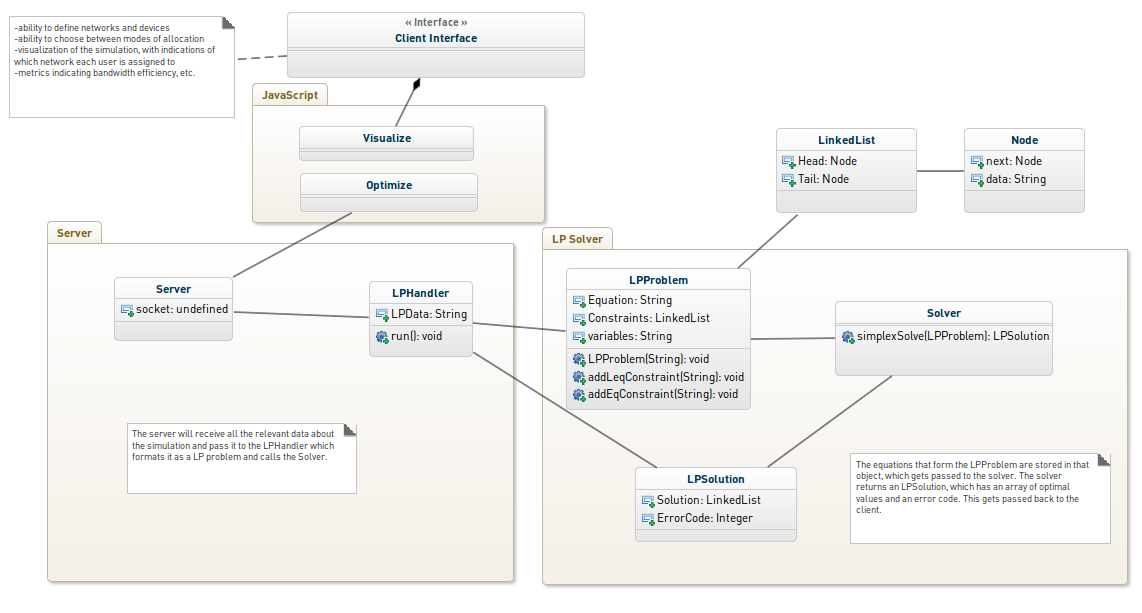
\includegraphics[width=600px, angle=270]{model.png}

\end{center}
\section{Implementation of the Linear Programming Solver}

~\indent Our Linear Programming solver uses the Two Phase 
Simplex Method \cite{chvatal83} to solve any feasible, bounded optimization problem in standard form, and does so without too much complexity in the codebase. The trade-off for this is that the efficiency likely doesn't compare to that of long-running commercially available and open source projects of a similar nature.
    \subsection{Input}
~\indent Our solver handles problems in the form:
\begin{eqnarray*}
\mbox{maximize}& \sum\limits_{j=1}^n c_jx_j\\
\mbox{subject to}& \sum\limits_{j=1}^n a_{ij}x_j \leq b_i\mbox{\ \ }(i \in I)\\
& \sum\limits_{j=1}^n a_{ij}x_j = b_i\mbox{\ \ }(i \in E)
\end{eqnarray*}

~\indent Since minimization problems can be written as maximizations by negating each variable, and similarly $\geq$ constraints can be negated to become $\leq$ ones, our solver only accepts three types of data:
\begin{enumerate}
\item precisely one objective equation with one or more decision variables (in its maximization form)
\item zero or more inequality constraints (in the $\leq$ form)
\item zero or more equality constraints
\end{enumerate}
...given that there is at least one constraint of some kind (otherwise the problem is unbounded).\\
The solver assumes the input to it is formatted correctly since that is handled on the server-side.

\subsection{Algorithm}
\textbf{Phase I}\\
~\indent If there are no equality constraints and all inequality constraints have positive b-values (they are $\leq$ not $\geq$), Phase I is skipped and the standard Simplex algorithm is applied. Otherwise, an auxiliary problem is formed to test the feasibility of the original problem. Namely,
\begin{eqnarray*}
\mbox{maximize}& \sum\limits_{i=1}^m (-x_{n+i})\\
\mbox{subject to}& \sum\limits_{j=1}^n a_{ij}x_j + w_ix_{n+i} \leq b_i\mbox{\ \ }(i \in I)\\
 & \sum\limits_{j=1}^n a_{ij}x_j + w_ix_{n+i} = b_i\mbox{\ \ }(i \in E)\\
 & \sum\limits_{j=1}^n a_{ij}x_j - w_ix_{n+i} = b_i\mbox{\ \ }(i \in E)\\
 & x_{n+i} \geq 0\mbox{\ \ }(i = 1, 2,...,m)
\end{eqnarray*}
given that $w_i = 1$ whenever $b_i \geq 0$ and $w_i = -1$ whenever $b_i < 0$ and with $m$ being the number of constraint equations and $n$ being the number of decision variables. Once this table is formed, the following steps are performed.
\begin{enumerate}
\item For all equations where $b_i < 0$, multiply the row by -1.
\item For every column, sum all rows except the objective equation and subtract this value from the objective equation coefficient in that column.
\item Calculate an upper bound on the number of iterations, specifically $e \choose l$, where $e$ is the number of candidates for entering the basis (the number of columns) and $l$ is the number of candidates for leaving it (the number of rows). 
\item Loop through the following code until we've either solved the problem (all objective equation coefficients are nonnegative) or exceeded the aforementioned maximum iterations.
  \begin{enumerate}
  \item Choose the column with the most negative objective equation coefficient as the pivot column.
  \item Choose the row in that column with the smallest positive $\frac{b_i}{a_{ij}}$ as the pivot row.
  \item Pivot on that column and row by dividing every entry in the pivot row by the value at the intersection of the pivot row and column, and then multiplying every other row by a suitable multiple of the pivot row such that their value in the pivot column becomes zero.
  \end{enumerate}
\item If the related problem's solution is 0, transfer the first $m$ rows and $n+m$ columns of the auxilary problem's table to the original table, as well as the objective equation's row.
\end{enumerate}

\noindent \textbf{Phase II}\\
Given that Phase I indicated the problem is solvable, start from the Basic Feasible Solution (BFS) given by Phase I and implement the standard simplex method to optimize it, looping through the following steps:
\begin{enumerate}
\item If the table was produced by Phase I, choose the minimum objective equation coefficient as the pivot column. Otherwise, choose the maximum. A nonnegative minimum in the former case or a nonpositive maximum in the latter indicate a solved problem.
\item If all entries in the pivot column are $\leq 0$, the problem is unbounded. Otherwise, the row in that column with the smallest positive $\frac{b_i}{a_{ij}}$ is the pivot row.
\end{enumerate}
If a solution was found, all decision variables are assumed to have the value 0 unless their column $i$ contains exactly one 1 and the rest 0's, in which case that row's $b_i$ value is the value of that decision variable in the optimal solution. These values and the optimal value of the objective equation are returned to the calling program.

\section{Questions}

\begin{itemize}
\item Is it necessary to duplicate each equality constraint in Phase I with opposite values for the artificial variables, $w_{n+i}$? Would we have to change anything else in our process if we removed that step?
\item Is it safe to delete all artificial variable columns at the end of Phase I, regardless of if they're in the basis at that point, or do they have to be pivoted out of the basis to maintain feasibility?
\end{itemize}

\section{Further Work}

~\indent In the near-term future, we are going to implement a web interface for the heterogeneous network simulator, which will allow the user to specify parameters and visualize the system's allocations. Longer-term, the project may be extended to a larger problem domain. For example, more allocation algorithms could be added.

\begin{thebibliography}{1}
\bibitem{chvatal83}
  Vašek Chvátal,
  Linear Programming.
  W. H. Freeman and Company, New York,
  1983.
\end{thebibliography}  
       
\end{document}
